\documentclass[tikz,border=5pt]{standalone}
\usepackage{amsmath}
\usetikzlibrary{arrows.meta,positioning,calc}

\begin{document}
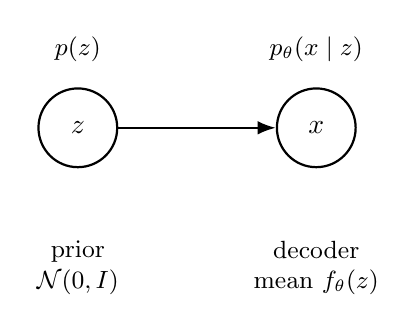
\begin{tikzpicture}[
    >=Latex,
    node distance=18mm and 20mm,
    var/.style={draw, circle, thick, minimum size=10mm, inner sep=0pt},
    plate/.style={draw, rounded corners, thick, inner sep=6pt},
    label/.style={font=\small},
]

\node[var] (z) {$z$};
\node[var, right=of z] (x) {$x$};

\draw[->, thick] (z) -- (x);

\node[label, above=2mm of z] {$p(z)$};
\node[label, above=2mm of x] {$p_\theta(x\mid z)$};

\node[label, below=8mm of z, align=center] {prior\\$\mathcal N(0,I)$};
\node[label, below=8mm of x, align=center] {decoder\\mean $f_\theta(z)$};

\end{tikzpicture}
\end{document}


